\chapter{Continuous Dynamics and Variational Networks}
\label{ch:continuous_dynamics}

In Chapter \ref{ch:unrolling} we explored the paradigm of algorithm unrolling, a highly effective technique that bridges the gap between classical iterative optimisation and deep learning. By unrolling a finite number of iterations of an algorithm like proximal gradient descent (see Algorithm \ref{alg:pgd}), we replaced hand-crafted parameters with learnable components. This yielded architectures that maintain a connection to the underlying physics of inverse problems whilst heavily leveraging the expressivity of data-driven methods.

However, unrolling generic optimisation algorithms leaves several theoretical and practical questions unanswered. As we increase the number of unrolled iterations to improve reconstruction accuracy, we hit a severe computational bottleneck: Backpropagation Through Time (BPTT) requires storing the intermediate activations of every layer in memory, which scales linearly with depth. For large-scale 3D inverse problems, this quickly exceeds the memory capacity of modern hardware. Furthermore, relying on discrete iterative steps obscures the underlying continuous physics of the learning process.

This chapter addresses these challenges by initiating a profound perspective shift. We will reframe deep learning not as a sequence of discrete algebraic layers, but as a problem of continuous dynamical systems. By taking the infinitesimal limit of deep residual networks, we arrive at continuous-time Ordinary Differential Equations (ODEs). This perspective elegantly transforms the training of neural networks into an \emph{optimal control problem}. We will formally derive the optimality conditions for this continuous framework, study symplectic numerical discretisations via Runge-Kutta methods, and finally apply these continuous control principles to Variational Networks for medical imaging to resolve phenomena such as the early stopping paradox.

\section{The Continuous Limit: Deep Learning as Dynamical Systems}
\label{sec:continuous_limit}

Traditionally, deep neural networks are built by stacking discrete layers. An input signal is iteratively transformed as it passes through sequential computational blocks. However, when this compositional approach is pushed to an infinitesimal limit, deep learning can be fundamentally reframed as a problem of continuous dynamical systems \cite{e2017proposal,haber2017stable}.

\subsection{Layer Transitions and Stability}

To understand this continuous limit, we first examine the mathematical structure of a single discrete neural network layer. A generic layer transition can be modelled as
\begin{equation}
    u^{l+1} = G\left(h(u^l) + \mathcal{F}(u^l, \Theta_l)\right) \, ,
    \label{eq:generic_layer}
\end{equation}
where $u^l \in \mathbb{R}^d$ is the input state vector at layer $l$, $\Theta_l$ are the learnable parameters (weights and biases) associated with that layer, and $G$ and $h$ are specific mapping functions (such as non-linear activations or normalisation operators), cf. \cite{haber2017stable}. 

When stacking these generic layers to create exceptionally deep networks, a critical numerical pathology emerges: the exploding or vanishing gradient problem. For a deep network to remain trainable via gradient descent, the mapping from layer $l$ to $l+1$ must remain stable. Mathematically, this implies that the gradient of the right-hand side of Equation \eqref{eq:generic_layer} with respect to $u^l$ must be close to the identity matrix, i.e.,
\begin{equation*}
    \nabla G \nabla h \sim I \, .
\end{equation*}
If the eigenvalues of this Jacobian deviate significantly from one, perturbations will either decay to zero or grow exponentially as they propagate through the depth of the network.

Residual Networks (ResNets) naturally fulfil this stability condition. By defining the transition such that $G(x) = x$ and $h(x) = x$, the ResNet update rule becomes a simple additive perturbation to the identity map (cf. Equation \eqref{eq:resnet_block}):
\begin{equation}
    u^{l+1} = u^l + \mathcal{F}(u^l, \Theta_l) \, .
    \label{eq:resnet_discrete}
\end{equation}
This architectural choice ensures that $\nabla_{u^l} u^{l+1} = I + \nabla_{u^l} \mathcal{F}(u^l, \Theta_l)$, which strongly regularises the flow of gradients and allows for the training of networks with hundreds of layers (cf. \cite{haber2017stable, e2017proposal}).

\subsection{Continuous ODE Formulation}

The discrete ResNet transition in Equation \eqref{eq:resnet_discrete} reveals a deep connection to numerical analysis. Let us rewrite the update rule slightly by artificially introducing a step size $\Delta t = 1$, i.e.,
\begin{equation*}
    \frac{u^{l+1} - u^l}{\Delta t} = \mathcal{F}(u^l, \Theta_l) \, .
\end{equation*}
This algebraic manipulation shows that the ResNet layer is exactly the \emph{forward Euler discretisation} of a continuous ordinary differential equation. We can imagine the discrete layer index $l$ mapping to a continuous time equivalent $t_l = l \Delta t$. If we allow the step size $\Delta t \to 0$ and the number of layers to approach infinity (whilst keeping the total "network time" horizon $T$ fixed), the sequence of hidden states $u^l$ transitions into a continuous trajectory $u(t)$. Similarly, the discrete parameters $\Theta_l$ are replaced by a continuous control variable $\Theta(t)$. By taking the infinitesimal limit, the difference quotient on the left-hand side becomes a time derivative, governed by the initial value problem
\begin{equation*}
    \frac{d}{dt}u(t) = \mathcal{F}\left(u(t), \Theta(t)\right) \quad \text{for } t \in [0, T] \, ,
\end{equation*}
with the initial condition $u(0) = u_0$, where $u_0$ is the input data. Here, $\Theta(t)$ represents the continuous control parameters (the time-dependent network weights and biases) acting over a fixed network time horizon $T$ \cite{e2017proposal, haber2017stable, benning2019deep}.

\subsection{Overcoming Instability}

Framing network architectures as discretised ODEs is not merely a theoretical curiosity; it provides a rigorous mathematical framework for designing stable architectures. By interpreting the forward pass as the integration of an ODE, we ensure that the learning problem remains well-posed. If the vector field $\mathcal{F}(u, \Theta(t))$ is appropriately constrained, the flow of the network remains bounded and stable from the initial input state $u(0)$ to the final output state $u(T)$. This continuous perspective systematically overcomes the numerical instabilities inherent in standard derivative-based learning algorithms.

\section{Deep Learning as Continuous Optimal Control}
\label{sec:optimal_control}

By formally interpreting the neural network as a continuous dynamical system, the supervised training process is mathematically transformed into an optimal control problem \cite{benning2019deep, e2017proposal}. Rather than finding a discrete set of matrices to minimise a sum, our objective is to find an optimal continuous control trajectory $\Theta(t)$ that steers the dynamical system to a desired terminal state at time $t=T$.

This continuous perspective offers several profound advantages over the discrete layer-by-layer view. Firstly, it allows us to decouple the learning problem (finding the optimal continuous trajectory) from the discretisation (how we numerically compute the forward pass on a computer). Secondly, it immediately connects deep learning to the established mathematical field of \href{https://en.wikipedia.org/wiki/Optimal_control}{optimal control theory}, giving us access to powerful analytical tools like the \href{https://en.wikipedia.org/wiki/Pontryagin%27s_maximum_principle}{Pontryagin Maximum Principle}.

\subsection{Cost Functional and Constraints}

In classical deep learning, as discussed in Section \ref{sec:deep-learning}, we seek to minimise an empirical risk function over a set of learnable parameters. In our continuous optimal control framework, this objective is generalised via a generic cost functional over the entire time horizon $[0, T]$. We define the cost functional $\mathcal{J}$ to encompass both a terminal cost component (measuring how well the final state $u(T)$ performs our task, like classification or regression) and a running cost explicitly regularising the control parameters over time, i.e.,
\begin{equation}
    \min_{\Theta, u} \left\{ \mathcal{J}(u(T), \Theta) := \mathcal{M}(u(T)) + \int_0^T \mathcal{R}(u(t), \Theta(t)) \, dt \right\} \, ,
    \label{eq:generic_cost_functional}
\end{equation}
where $\mathcal{M}$ acts as the terminal cost and $\mathcal{R}$ specifies the regularisation function or running cost. This minimisation is subject to the fundamental ODE constraint governing the continuous state evolution, i.e.,
\begin{equation*}
    \frac{d}{dt}u(t) = \mathcal{F}\left(u(t), \Theta(t)\right) \quad \text{for } t \in (0, T], \quad \text{with initial condition} \quad u(0) = u_0 \, .
\end{equation*}

Here, $u(t) \in \mathcal{U}$ belongs to the state space $\mathcal{U}$, and the control sequence $\Theta(t) \in \mathcal{P}$ belongs to an admissible parameter class $\mathcal{P}$. The function $\mathcal{F}$ characterises how the control interacts with the state space at infinitesimally small propagation steps along the continuous horizon.

\begin{exm}[Training a classifier on data]
Connecting back to the supervised learning paradigm introduced in Section \ref{sec:dnn-training}, suppose we have a dataset comprised of $m$ input-output pairs $(x_i, y_i) \in \mathbb{R}^d \times \mathbb{R}$. We can construct the terminal cost function $\mathcal{M}$ corresponding to empirical risk minimisation (cf. Equation \eqref{eq:dnn-empirical-risk-minimisation}) over continuous control parameters $\Theta(t)$, terminal weights $W$, and scalar bias $\mu$ for the application of classification via
\begin{align*}
    \mathcal{M}(u(T)) &:= \frac{1}{m} \sum_{i=1}^m \left| \mathcal{C}\left(W u_i(T) + \mu\right) - y_i \right|^2 \, ,
\end{align*}
where $\mathcal{C}$ is a hypothesis or activation function, and $W$ and $\mu$ are additional learnable parameters mapping the final state to our target output. We commonly employ a Tikhonov regularisation penalty over continuous time by choosing
\begin{align*}
    \mathcal{R}(u(t), \Theta(t)) &:= \frac{\lambda}{2} \|\Theta(t)\|_2^2 \, .
\end{align*}
Plugging these into \eqref{eq:generic_cost_functional}, the optimal control problem specifically for this learning task takes the form
\begin{equation*}
    \min_{\Theta, u, W, \mu} \left\{ \frac{1}{m} \sum_{i=1}^m \left| \mathcal{C}\left(W u_i(T) + \mu\right) - y_i \right|^2 + \frac{\lambda}{2} \int_0^T \|\Theta(t)\|_2^2 \, dt \right\} \, ,
\end{equation*}
subject to $\frac{d}{dt}u_i(t) = \mathcal{F}(u_i(t), \Theta(t))$ and $u_i(0) = x_i$ for all $i=1,\dots,m$.
\end{exm}
To visualise this continuous transformation, we can apply this optimal control framework to standard 2D binary classification tasks, such as separating concentric rings or interleaved spirals. The initial state $u(0)$ represents the 2D coordinates of the data points. As the continuous network time $t$ progresses to $T$, the learned optimal control trajectory $\Theta(t)$ dynamically transforms the state space, warping the geometry of the data points over time until they are linearly separable by the terminal weights $W$.

\begin{figure}[htpb]
    \centering
    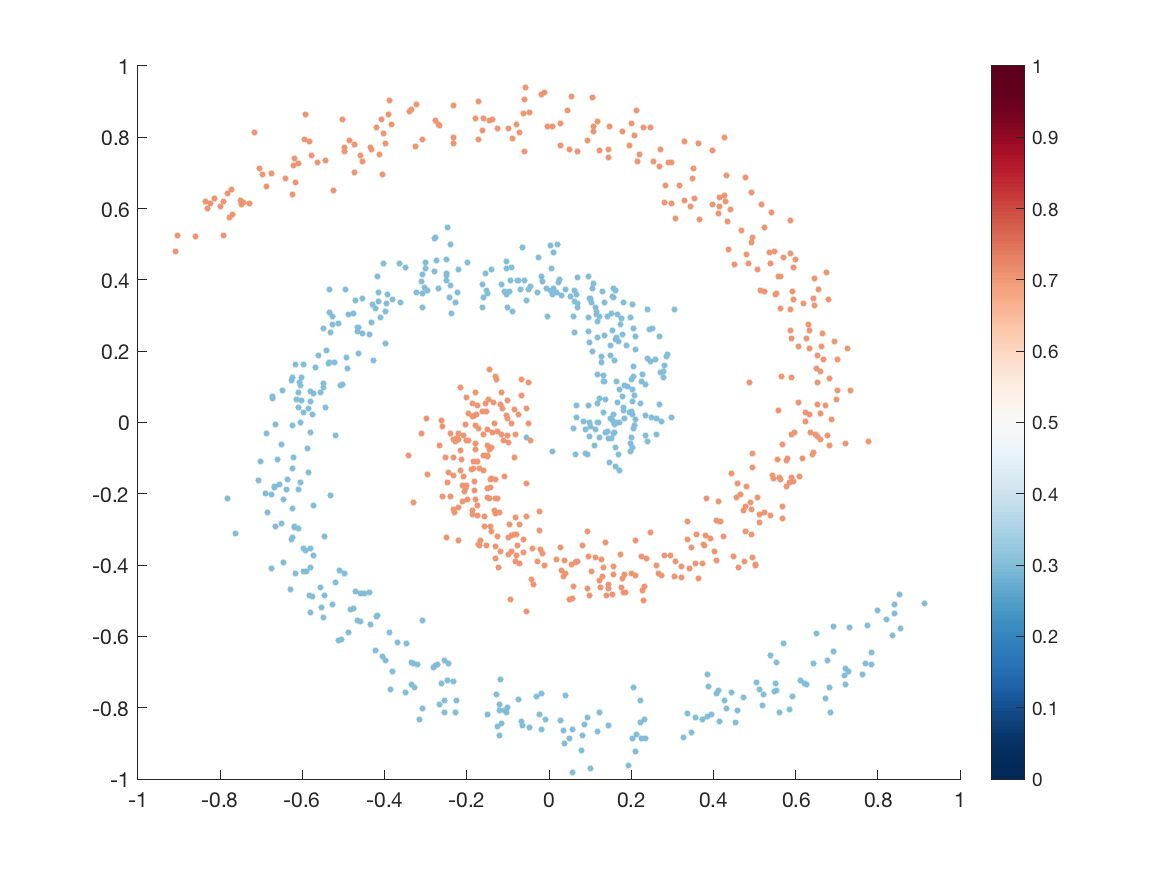
\includegraphics[width=0.4\textwidth]{../Common_Images/optimalcontrol/example_spiral2d} 
    \caption{An example of a 2D binary classification toy dataset (spirals) where deep learning as continuous optimal control can be naturally visualised. The network learns a flow that disentangles the two classes over the time horizon $T$. Image taken from \cite{benning2019deep}.}
    \label{fig:toy_data}
\end{figure}

\begin{figure}[htpb]
    \centering
    \begin{subfigure}[b]{0.24\textwidth}
        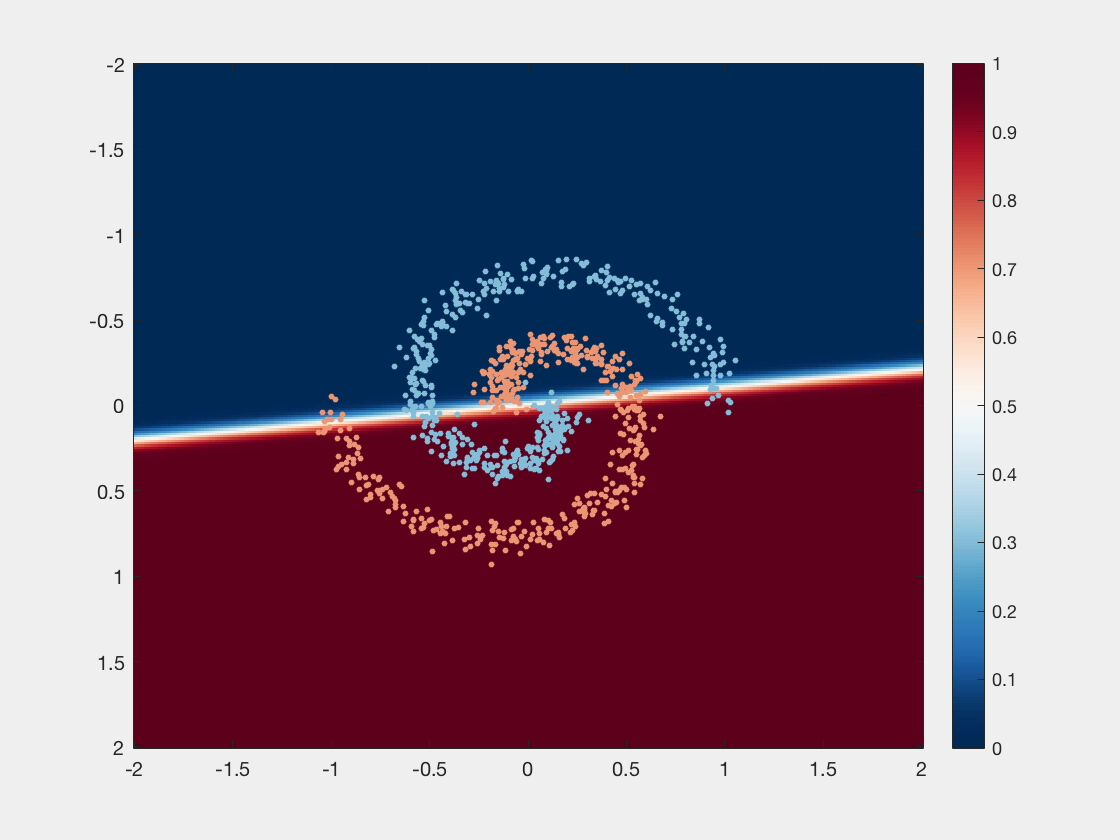
\includegraphics[width=\textwidth]{../Common_Images/optimalcontrol/ResNet_squared_seed1_video_01}
        \caption{Time $t=0$}
    \end{subfigure}
    \hfill
    \begin{subfigure}[b]{0.24\textwidth}
        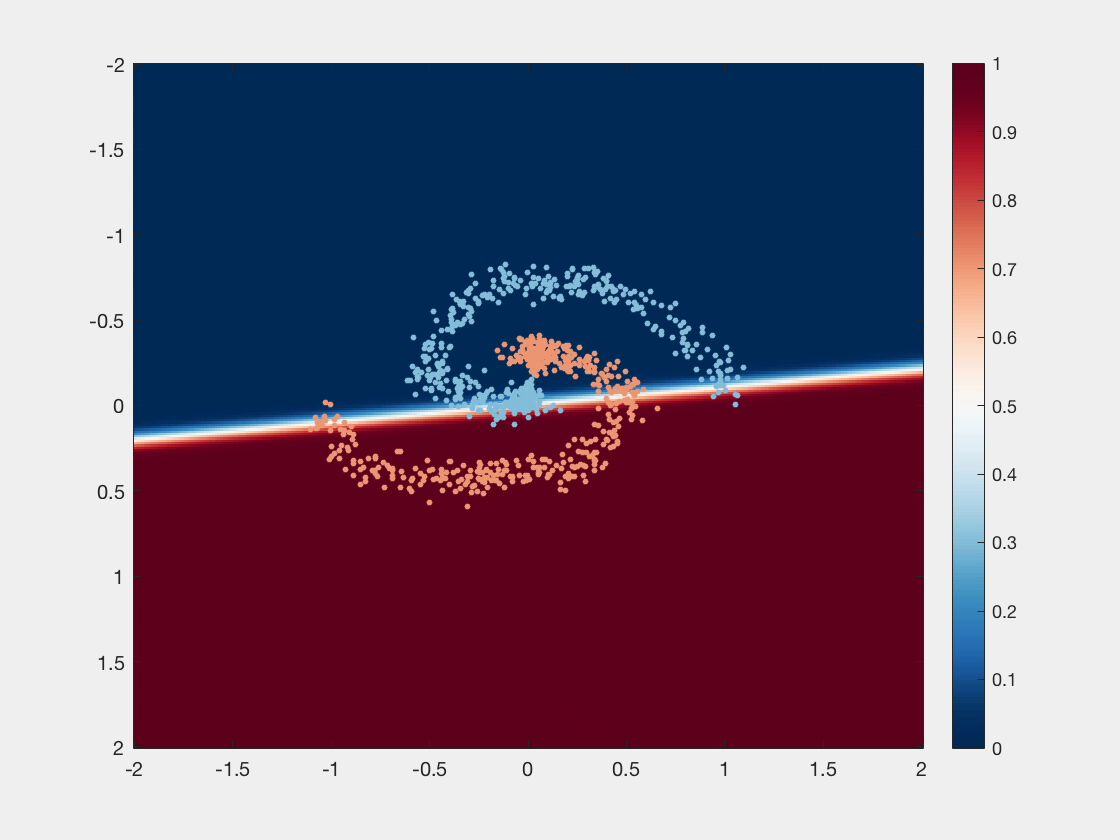
\includegraphics[width=\textwidth]{../Common_Images/optimalcontrol/ResNet_squared_seed1_video_08}
        \caption{Time $t \approx T/3$}
    \end{subfigure}
    \hfill
    \begin{subfigure}[b]{0.24\textwidth}
        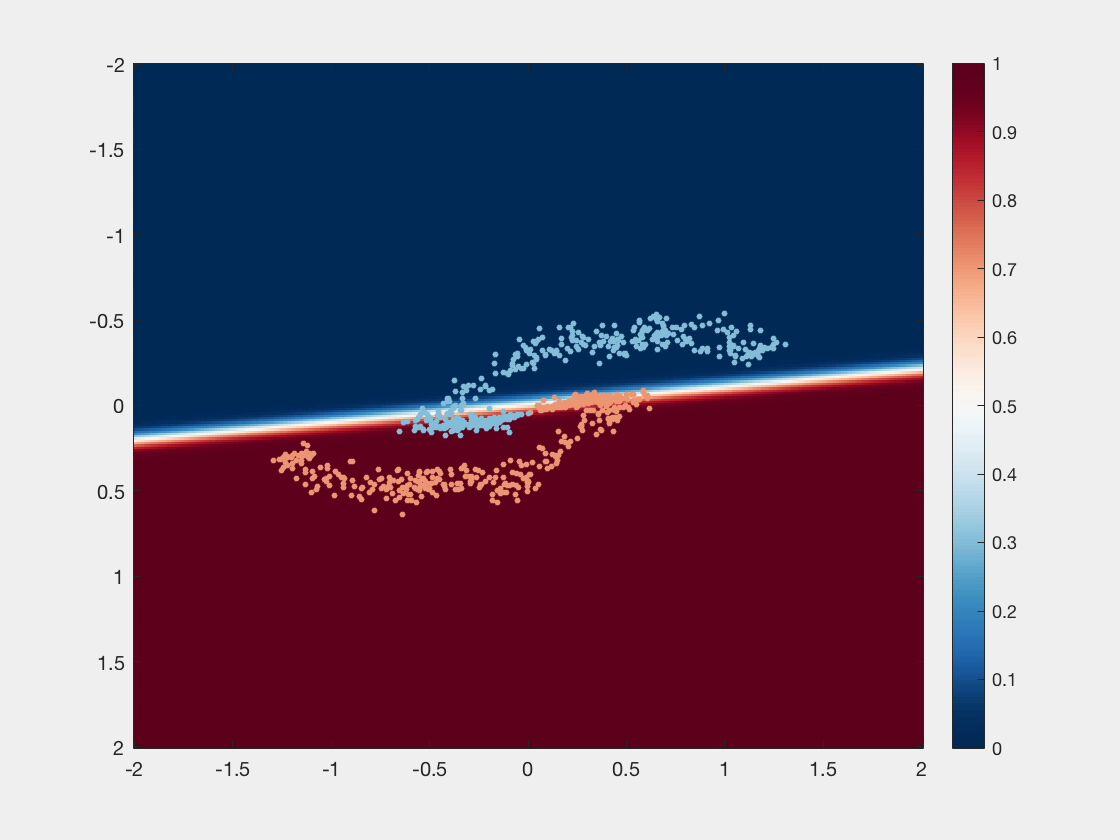
\includegraphics[width=\textwidth]{../Common_Images/optimalcontrol/ResNet_squared_seed1_video_15}
        \caption{Time $t \approx 2T/3$}
    \end{subfigure}
    \hfill
    \begin{subfigure}[b]{0.24\textwidth}
        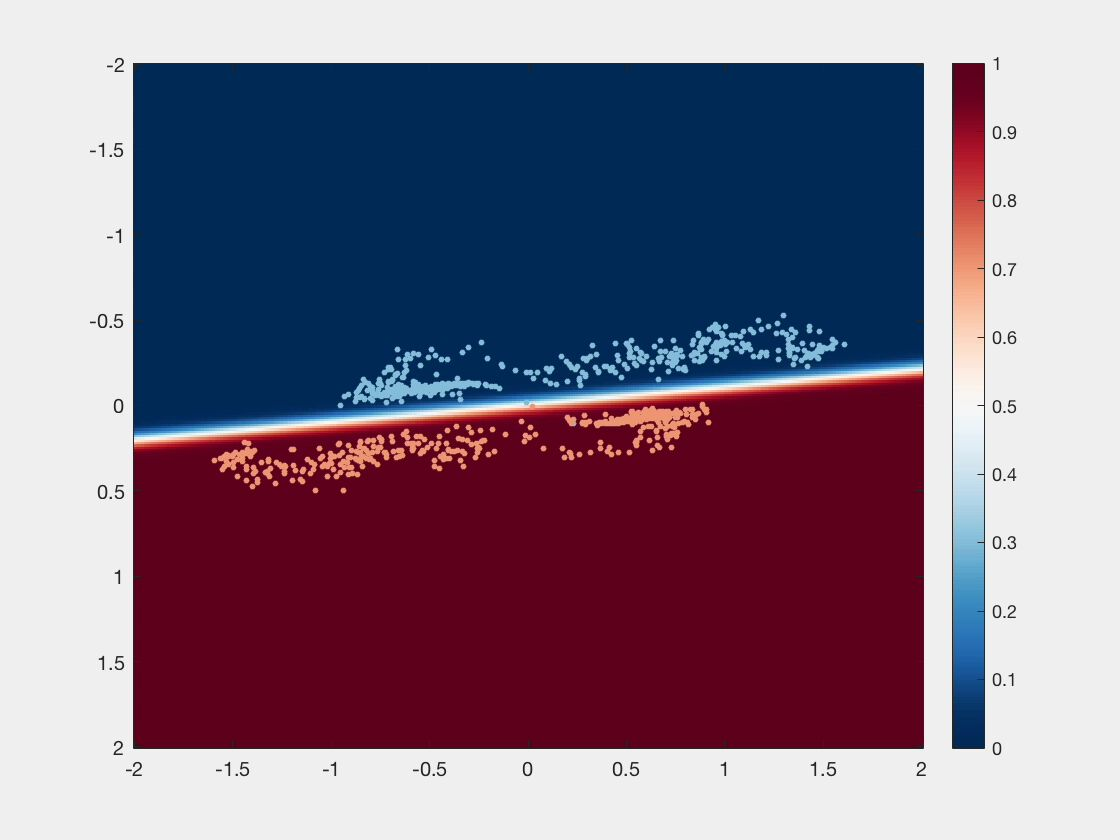
\includegraphics[width=\textwidth]{../Common_Images/optimalcontrol/ResNet_squared_seed1_video_21}
        \caption{Terminal Time $t=T$}
    \end{subfigure}
    \caption{Progression of state space transformation across the continuous horizon using a ResNet (Forward Euler) flow. The optimal control parameters continuously stretch and unwrap the initially tangled spiral classes until they are neatly partitioned and linearly separable. Images taken from \cite{benning2019deep}.}
    \label{fig:resnet_spiral_warping}
\end{figure}

\subsection{The Lagrangian Formulation}

To perform gradient-based numerical optimisation, we need to know how the final cost $\mathcal{J}$ reacts to continuous changes in the control signal $\Theta(t)$. Rather than calculating this via standard variational calculus and chain rules -- which can become algebraically cumbersome -- we can employ \emph{Lagrange multipliers}, staying mathematically consistent with the constrained optimisation techniques (such as ADMM and PDHG) introduced in Chapters \ref{ch:unrolling} and \ref{ch:pnp}. Since the state $u(t)$ is tightly constrained by the dynamical system $\frac{d}{dt}u(t) = \mathcal{F}(u(t), \Theta(t))$, we can elegantly reformulate the constrained optimal control problem into an unconstrained saddle-point problem.

We introduce a continuous-time Lagrange multiplier $p(t) \in \mathcal{U}$, which in optimal control terminology is referred to as the \emph{adjoint state} (or co-state). The Lagrangian functional $\mathcal{L}(u, \Theta, p)$ is defined by appending the ODE constraint to the generic cost functional \eqref{eq:generic_cost_functional} via an $L^2$-inner product integrated over the entire time horizon, i.e.,
\begin{align}
    \begin{split}
    \mathcal{L}(u, \Theta, p) &:= \mathcal{M}\left(u(T)\right) + \int_0^T \mathcal{R}\left(u(t), \Theta(t)\right) \, dt \\
    &\quad - \int_0^T \left\langle p(t), \frac{d}{dt}u(t) - \mathcal{F}\left(u(t), \Theta(t)\right) \right\rangle_{\mathcal{U}} \, dt \, .
    \end{split}\label{eq:optcontrollag}
\end{align}
To make it easier to take derivatives with respect to $u(t)$, we isolate $u(t)$ from its time derivative by applying integration by parts to the first half of the constraint integral, to obtain
\begin{equation}
    \int_0^T \left\langle p(t), \frac{d}{dt}u(t) \right\rangle_{\mathcal{U}} \, dt = \langle p(T), u(T) \rangle_{\mathcal{U}} - \langle p(0), u(0) \rangle_{\mathcal{U}} - \int_0^T \left\langle \frac{d}{dt}p(t), u(t) \right\rangle_{\mathcal{U}} \, dt \, .\label{eq:optcontrolopt}
\end{equation}
Substituting \eqref{eq:optcontrolopt} into the Lagrangian \eqref{eq:optcontrollag} yields the equivalent formulation
\begin{align*}
    \mathcal{L}(u, \Theta, p) &= \mathcal{M}\left(u(T)\right) - \langle p(T), u(T) \rangle_{\mathcal{U}} + \langle p(0), u_0 \rangle_{\mathcal{U}} \\
    &\quad + \int_0^T \left[ \mathcal{R}\left(u(t), \Theta(t)\right) + \left\langle \frac{d}{dt}p(t), u(t) \right\rangle_{\mathcal{U}} + \left\langle p(t), \mathcal{F}\left(u(t), \Theta(t)\right) \right\rangle_{\mathcal{U}} \right] \, dt \, ,
\end{align*}
where the time derivative acts on the adjoint state $p(t)$ instead of $u(t)$. Here we have explicitly used the initial condition $u(0) = u_0$.

\subsection{First-Order Optimality Conditions}

With the unconstrained Lagrangian established, the necessary first-order optimality conditions simply require the derivatives of $\mathcal{L}$ with respect to all three variables -- $p$, $u$, and $\Theta$ -- to vanish. 

First, taking the gradient with respect to the multiplier $p(t)$ simply recovers our original state equation
\begin{equation*}
    \nabla_p \mathcal{L} = 0 \quad \implies \quad \frac{d}{dt}u(t) = \mathcal{F}\left(u(t), \Theta(t)\right) \, , \quad u(0) = u_0 \, .
\end{equation*}

Next, we take the variation with respect to the state variable $u$. Because $u$ appears both at the terminal time $T$ and inside the integral over $(0, T)$, we obtain two coupled conditions. For the terminal boundary, the variation with respect to $u(T)$ dictates
\begin{equation*}
    \nabla_{u(T)} \mathcal{L} = 0 \quad \implies \quad \nabla_u \mathcal{M}\left(u(T)\right) - p(T) = 0 \quad \implies \quad p(T) = \nabla_u \mathcal{M}\left(u(T)\right) \, ,
\end{equation*}
which is the terminal condition for the adjoint state. For the continuous interval $(0, T)$, calculating the variation of the integrand with respect to $u(t)$ (and using the adjoint operator definition $\langle p, \partial_u \mathcal{F} \delta u \rangle = \langle (\partial_u \mathcal{F})^* p, \delta u \rangle$) yields the adjoint equation
\begin{equation*}
    \nabla_{u(t)} \mathcal{L} = 0 \quad \implies \quad \frac{d}{dt}p(t) + \left(\partial_u \mathcal{F}(u(t), \Theta(t))\right)^* p(t) + \nabla_u \mathcal{R}\left(u(t), \Theta(t)\right) = 0 \, .
\end{equation*}
Rearranging this, we see that the adjoint state evolves backwards in time, i.e.,
\begin{equation*}
    -\frac{d}{dt} p(t) = \left(\partial_u \mathcal{F}(u(t), \Theta(t))\right)^* p(t) + \nabla_u \mathcal{R}\left(u(t), \Theta(t)\right) \, ,
\end{equation*}
serving as the continuous-time analogue of discrete backpropagation.

Finally, taking the variation with respect to the continuous control parameters $\Theta(t)$ isolates the gradient we need for learning. For an optimal control trajectory, this derivative must be exactly zero:
\begin{equation}
    \nabla_{\Theta(t)} \mathcal{L} = 0 \quad \implies \quad \left(\partial_\Theta \mathcal{F}(u(t), \Theta(t))\right)^* p(t) + \nabla_\Theta \mathcal{R}\left(u(t), \Theta(t)\right) = 0 \quad \text{for } t \in [0, T] \, .
    \label{eq:grad_p_zero}
\end{equation}
During gradient-based training, if we have not yet converged to the optimal parameters, the left-hand side of Equation \eqref{eq:grad_p_zero} directly supplies the continuous gradient $\nabla_{\Theta(t)} \mathcal{J}$ required to equivalently update $\Theta(t)$.

\subsection{The Hamiltonian and Pontryagin's Minimum Principle}

The optimal control problem described above naturally gives rise to defined energy systems by grouping key components. To further align the deep learning problem with physical theories like classical mechanics, we encapsulate the required equations in a single functional called the \emph{Hamiltonian}, $\mathcal{H}: \mathcal{U} \times \mathcal{U} \times \mathcal{P} \to \mathbb{R}$, via
\begin{equation*}
    \mathcal{H}\left(u(t), p(t), \Theta(t)\right) := \left\langle p(t), \mathcal{F}\left(u(t), \Theta(t)\right) \right\rangle_{\mathcal{U}} + \mathcal{R}\left(u(t), \Theta(t)\right) \, .
\end{equation*}
By directly computing the partial derivatives of the Hamiltonian, we recover the foundational set of continuous first-order optimality conditions
\begin{align*}
    \frac{d}{dt} u(t) &= \nabla_p \mathcal{H}\left(u(t), p(t), \Theta(t)\right) &\quad (\text{State Equation}) \\
    -\frac{d}{dt} p(t) &= \nabla_u \mathcal{H}\left(u(t), p(t), \Theta(t)\right) &\quad (\text{Adjoint Equation}) \\
    0 &= \nabla_\Theta \mathcal{H}\left(u(t), p(t), \Theta(t)\right) &\quad (\text{Optimality Condition}) 
\end{align*}
with boundary conditions matching the initial input data $u(0) = u_0$ and the final cost derivative $p(T) = \nabla_u \mathcal{M}(u(T))$.

This theoretical architecture forms the backbone of \emph{Pontryagin's Minimum Principle}, stating that for a control trajectory to be optimal, the Hamiltonian defined must be strictly minimised across the state variables for almost every time $t \in [0, T]$. This produces a deterministic two-point boundary value problem. Because we have fixed boundaries at opposite sides of the temporal domain ($u(0)$ and $p(T)$), resolving the continuous parameter gradients necessitates solving the forward state ODE to evaluate $u(T)$, before the backward adjoint ODE can be integrated from $T$ down to $0$ \cite{benning2019deep}.

\section{Numerical Discretisation and ODE-Inspired Architectures}
\label{sec:numerical_discretisation}

To evaluate these continuous control problems computationally, a ``first-optimise-then-discretise'' approach is employed. Unlike standard deep learning -- which discretises first and calculates gradients via backpropagation -- this approach derives the continuous optimality conditions first and \emph{then} discretises them using numerical ODE solvers \cite{benning2019deep}.

\subsection{Symplectic Partitioned Runge-Kutta Methods}

As mentioned at the beginning of this chapter, in standard architectures such as ResNets, the transition from one layer to the next effectively constitutes a \emph{forward Euler} discretisation of the underlying ODE. While forward Euler is computationally inexpensive, it is a first-order method, meaning it requires exceptionally small time steps (and consequently, very deep networks) to achieve accurate and stable integration over a fixed horizon. By adopting more flexible Runge-Kutta (RK) methods, one achieves higher-order approximations, allowing for more complex transformations with fewer layers (or stages).

To formally introduce these methods, a generic $s$-stage Runge-Kutta scheme for the forward state equation $\frac{d}{dt}u = \mathcal{F}(u, \Theta)$ computes the next state $u^{l+1}$ via intermediate stages $U_i^l$:
\begin{subequations}
\label{eq:rk_state}
\begin{align}
    U_i^l &= u^l + \Delta t \sum_{j=1}^s a_{i,j} \mathcal{F}(U_j^l, \Theta_j^l) \, , \quad i = 1, \dots, s \, , \label{eq:rk_state_stage} \\
    u^{l+1} &= u^l + \Delta t \sum_{i=1}^s b_i \mathcal{F}(U_i^l, \Theta_i^l) \, . \label{eq:rk_state_update}
\end{align}
\end{subequations}
where $b_i$ are the weights and $a_{i,j}$ is the coefficient matrix. However, deep learning formulated as optimal control requires solving a coupled two-point boundary value problem: integrating the state $u(t)$ forward in time, and integrating the adjoint $p(t)$ backward in time. 

To handle this, we employ a \emph{Partitioned Runge-Kutta (PRK)} method. A PRK applies the RK scheme \eqref{eq:rk_state} to the forward state equation, and a distinct, matched RK scheme (with weights $\tilde{b}_i$ and matrix $\tilde{a}_{i,j}$) to the backward adjoint equation:
\begin{subequations}
\label{eq:rk_adjoint}
\begin{align}
    P_i^l &= p^l + \Delta t \sum_{j=1}^s \tilde{a}_{i,j} \ell_j^l \, , \quad i = 1, \dots, s \, , \label{eq:rk_adjoint_stage} \\
    p^{l+1} &= p^l + \Delta t \sum_{i=1}^s \tilde{b}_i \ell_i^l \, , \label{eq:rk_adjoint_update}
\end{align}
\end{subequations}
where $\ell_i^l = -\left(\partial_u \mathcal{F}(U_i^l, \Theta_i^l)\right)^* P_i^l$ represents the stage derivatives for the adjoint state.

Introducing advanced discretisations brings us to a structural challenge regarding how we compute gradients. There are two competing paradigms in numerical optimal control: the ``first-discretise-then-optimise'' approach (standard deep learning backpropagation through discrete layers) and the ``first-optimise-then-discretise'' approach (deriving the continuous adjoint equations first, then numerically discretising the resulting boundary value problem).

Remarkably, these two approaches perfectly commute if the chosen discretisation scheme is a \emph{symplectic} PRK method \cite{benning2019deep, hager2000runge}. For a PRK method to be symplectic, it must perfectly preserve the quadratic invariants of the Hamiltonian system. Specifically, the discrete inner product between the state variations $v^l$ and the adjoint states $p^l$ must remain constant, i.e., $\langle p^{l+1}, v^{l+1} \rangle = \langle p^l, v^l \rangle$. Ensuring this algebraic preservation strictly requires the coefficients of the paired RK schemes to satisfy
\begin{equation}
    b_i = \tilde{b}_i \quad \text{and} \quad b_i\tilde{a}_{i,j} + \tilde{b}_j a_{i,j} - b_i\tilde{b}_j = 0 \quad \text{for all } i, j = 1, \dots, s \, .
    \label{eq:symplectic_conditions}
\end{equation}

When these conditions inherently hold, applying the discretisation uniquely guarantees that the numerical gradients evaluated from the ``first-optimise'' continuous approach exactly match the true analytical gradients of the discretised loss function calculated via backpropagation \cite{hager2000runge, sanzserna2015sympletic}. Standard ResNet backpropagation automatically falls into this category, because the combination of an explicit forward Euler pass and an implicit backward Euler pass gracefully acts as a valid symplectic PRK method.

\begin{exm}[The Symplectic Euler Method]
To make these conditions concrete, consider the simplest symplectic PRK: the Symplectic Euler method. Rather than using the standard forward Euler for both passes, we pair the \emph{explicit} Euler method for the forward state with the \emph{implicit} Euler method for the backward adjoint state. 

For a single stage ($s=1$), the explicit forward Euler is defined by the weights $b_1 = 1$ and $a_{1,1} = 0$. To satisfy the symplectic conditions in Equation \eqref{eq:symplectic_conditions}, the backward method must use $\tilde{b}_1 = b_1 = 1$. The second condition requires $1 \cdot \tilde{a}_{1,1} + 1 \cdot 0 - 1 \cdot 1 = 0$, which mandates that $\tilde{a}_{1,1} = 1$ (the implicit Euler method). Applying this to our ODEs yields the discrete update rules:
\begin{align*}
    u^{l+1} &= u^l + \Delta t \, \mathcal{F}(u^l, \Theta^l) \, , \\
    p^{l+1} &= p^l - \Delta t \left(\partial_u \mathcal{F}(u^l, \Theta^l)\right)^* p^{l+1} \, , \\
    0 &= \left(\partial_\Theta \mathcal{F}(u^l, \Theta^l)\right)^* p^{l+1} \, .
\end{align*}
This pairing perfectly preserves the discrete Hamiltonian dynamics. In practice, higher-order explicit methods, such as the 2-stage Improved Euler or 4-stage Kutta methods, can be formulated into symplectic PRKs by algebraically deriving their corresponding backward coefficients to evaluate gradients accurately.
\end{exm}

\begin{table}[htpb]
    \centering
    \begin{tabular}{c|cc}
    0 & 0 & 0 \\ 
    1 & 1 & 0 \\ \hline
      & 1/2 & 1/2
    \end{tabular}
    \caption{Butcher tableau for the explicit 2-stage Improved Euler method. When used for the forward pass, a unique implicit backward tableau is derived via the symplectic conditions to ensure exact gradient matching.}
    \label{tab:improved_euler}
\end{table}

\subsection{ODENet and Learnable Time Steps}

By treating deep learning as an ODE, the ``time step'' $\Delta t$ between layers is no longer a fixed hyperparameter but can become a learnable parameter $\alpha$. In the \emph{ODENet} architecture, the control set is expanded to $\Theta = (W, \beta, \alpha)$, such that the flow is given by:
\begin{equation*}
    \mathcal{F}(u, \Theta) = \alpha \sigma(W u + \beta) \, .
\end{equation*}
This allows the network to dynamically adjust the integration step size, effectively optimising its own depth mapping \cite{benning2019deep}.

A powerful variation projects these learnable time steps $\alpha$ onto a probability simplex $\mathcal{S} = \{ \alpha \in \mathbb{R}^N \mid \alpha^{[j]} \ge 0, \sum_j \alpha^{[j]} = 1 \}$. This projection induces extreme sparsity. The network automatically sets most time steps to exactly zero, meaning it effectively uses only 2 to 3 active layers to solve complex transformations, severely reducing the online memory footprint during inference.

Empirically, freeing the time step from a fixed hyperparameter grid allows the ODENet to learn complex state space transformations much more aggressively. During training on 2D datasets, standard ODENets are often observed to learn negative time steps, introducing non-trivial, non-monotonic dynamics that allow for highly flexible feature transformations.

As illustrated in Figure \ref{fig:learned_timesteps}, when the simplex constraint $\mathcal{S}$ is applied, the network systematically drops unnecessary integration steps by setting their respective $\alpha^{[j]}$ to exactly zero. This effectively compresses a 20-layer network down to just 2 or 3 active transformational layers without sacrificing classification accuracy, verifying the optimal control hypothesis that network depth can be algorithmically learned.

\begin{figure}[htpb]
    \centering
    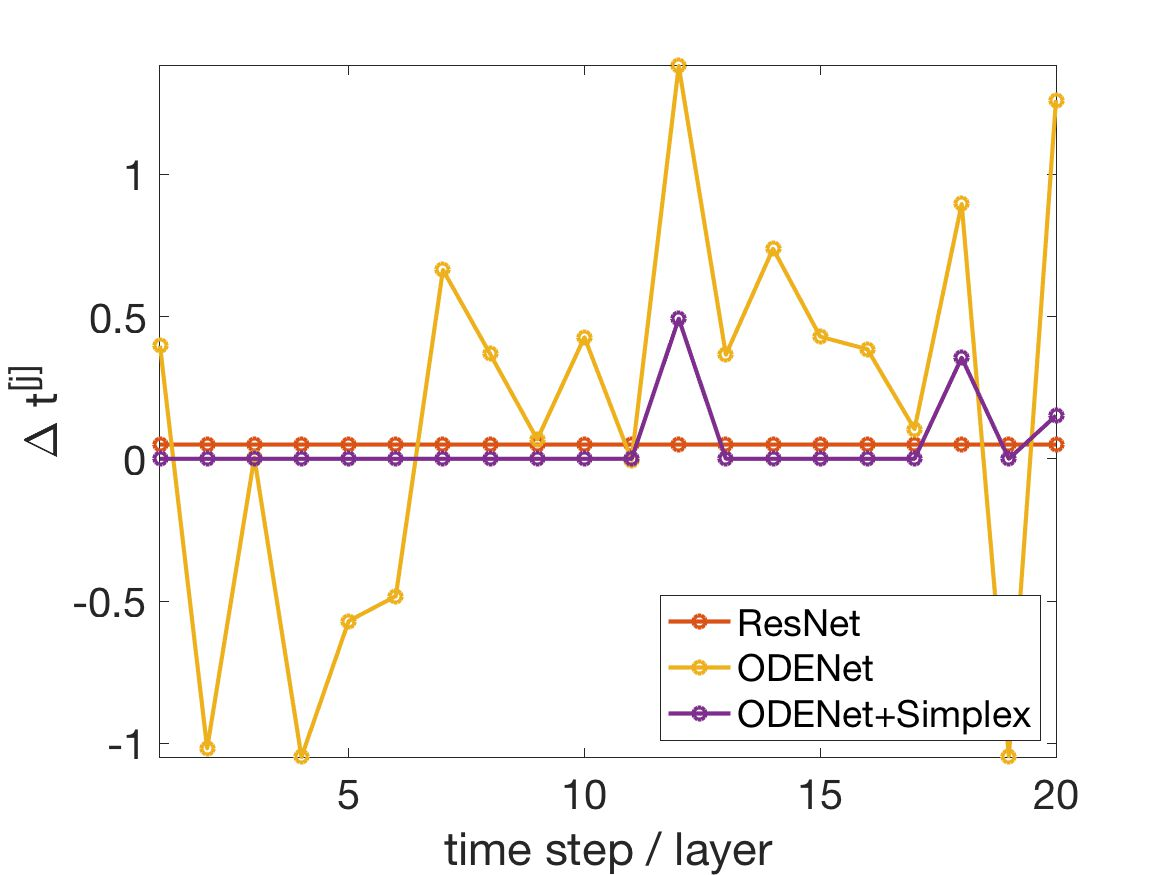
\includegraphics[width=0.7\textwidth]{../Common_Images/optimalcontrol/example_squares2d_20layers_backtracking1_seed1_timesteps}
    \caption{Learned time steps for ResNet (fixed at 1), ODENet, and ODENet+Simplex. The simplex constraint forces the network to automatically select only a few active layers, zeroing out the rest. Figure taken from \cite{benning2019deep}.}
    \label{fig:learned_timesteps}
\end{figure}

\section{Variational Networks: Bridging Energy Minimisation and Deep Learning}
\label{sec:vn_energy}

So far, we have seen how interpreting deep architectures like ResNets as discretised ODEs provides profound insights into their stability, depth, and training dynamics. This ODE-inspired perspective can also be applied in reverse: instead of analysing an existing artificial network as a continuous dynamical system, we can derive neural networks directly by discretising the continuous gradient flows of established physical energy functionals. This mathematically grounded approach is particularly powerful in the physical sciences for solving complex inverse problems like MRI reconstruction and image deblurring. By unrolling these continuous gradient descent processes into a sequence of network layers, we naturally arrive at Variational Networks (VNs) -- architectures that fuse the rigorous theoretical properties of variational models with the highly parameterised expressiveness of deep learning \cite{kobler2017variational,hammernik2018learning}.

\subsection{Energy Minimisation and the Field of Experts}

As introduced in Chapter \ref{ch:reg}, image reconstruction can be formulated as minimising an energy functional $E(u)$ consisting of a data fidelity term and a regularisation term. By heavily parameterising the regulariser using the Fields of Experts (FoE) framework from Equation \eqref{eq:foe_model}, the continuous energy functional takes the form
\begin{equation}
    E(u) = \frac{\lambda}{2} \|K u - f\|_2^2 + \sum_{i=1}^{N_D} \sum_{p=1}^N \rho_i\left((D_i u)_p\right) \, ,
    \label{eq:vn_energy}
\end{equation}
where $K$ is the forward operator (e.g., the Fourier transform combined with coil sensitivity maps in MRI), $f$ is the measured sensor data, and $\lambda$ controls the data fidelity weight and can be seen as a regularisation parameter (and the inverse of $\alpha$ in previous chapters). The FoE regulariser applies a set of $N_D$ learned convolutional filters $D_i$ to the image $u$. The filter responses at each pixel $p$ are then evaluated by a learned, non-linear potential function $\rho_i$ \cite{kobler2017variational}.

To enable highly flexible, data-driven activation functions, the derivatives of the potential functions, $\rho_i^\prime$, are parameterised as a weighted sum of $M$ Gau\ss ian Radial Basis Functions (RBFs), i.e.,
\begin{equation}
    \rho_i'(x) = \sum_{j=1}^M w_{ij} \exp\left(-\frac{(x - \mu_j)^2}{2\sigma^2}\right) \, ,
    \label{eq:rbf_activation}
\end{equation}
where $\mu_j$ are equidistant centers and $w_{ij}$ are the learnable weights \cite{hammernik2018learning}. 

\subsection{Incremental Gradient Steps}

To minimise the energy $E(u)$, we can unroll a gradient descent scheme (see Algorithm \ref{alg:pgd}). Calculating the derivative of Equation \eqref{eq:vn_energy} with respect to $u$ and formulating a discrete gradient descent step yields the fundamental update rule for a single Variational Network stage, which reads
\begin{equation}
    u^{t+1} = u^t - \left( \sum_{i=1}^{N_D} (D_i^t)^\top \rho_i^{t\prime}(D_i^t u^t) + \lambda^t K^*(K u^t - f) \right) \, ,
\end{equation}
for $t = 0, \dots, T-1$. Here, the parameters $\Theta^t = \{D_i^t, w_{ij}^t, \lambda^t\}$ are allowed to vary across each stage $t$, effectively increasing the capacity of the model and similar to unrolled architectures introduced in Chapter \ref{ch:unrolling}. 

\begin{figure}[p]
    \centering
    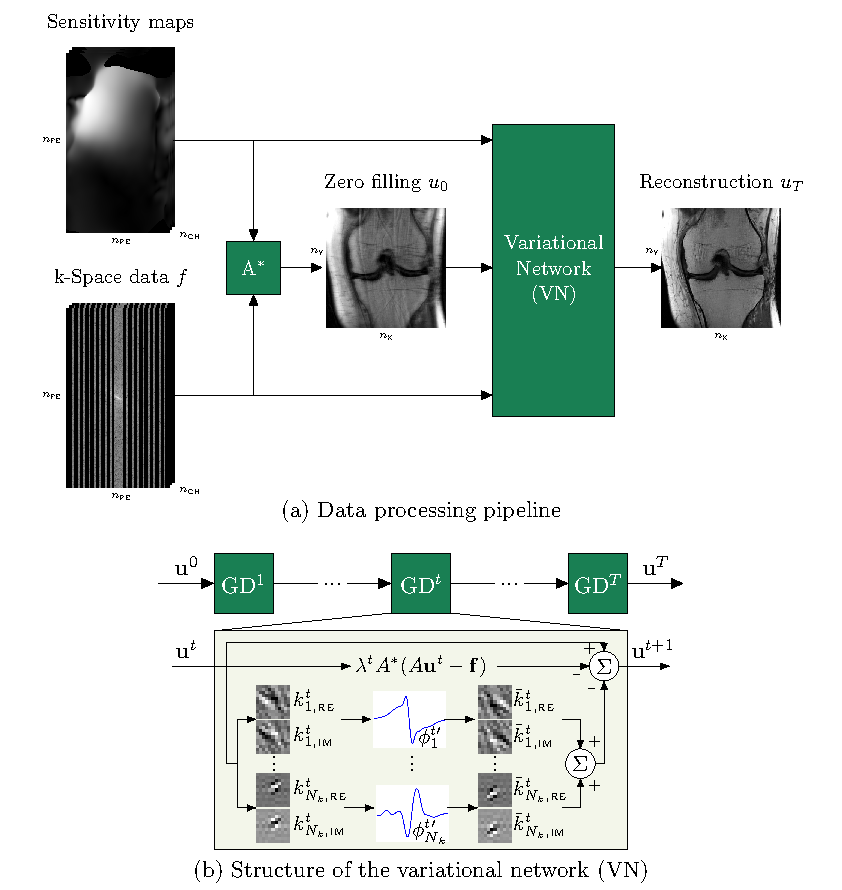
\includegraphics[width=1.0\textwidth]{../Common_Images/varnetworks/figure1-vn_overview}
    \caption{Overview of a Variational Network architecture. The network simulates an unrolled iterative scheme to minimise an energy functional where the gradient domain update acts equivalently to a residual block in a deep neural network. Image taken from \cite{hammernik2018learning}.}
    \label{fig:vn_overview}
\end{figure}

This structure exactly mirrors the computational architecture of deep Residual Networks (ResNets), where the data fidelity term acts as a skip connection enforcing physical consistency, and the regularisation term acts as a convolutional residual block. Training this architecture is a highly non-convex optimal control problem, which can be solved efficiently using algorithms such as the Inertial Incremental (Proximal) Gradient (IIPG) method, ensuring stable parameter updates across the unrolled stages \cite{hammernik2018learning}.

\subsection{Convex vs. Non-Convex Limits}

A profound theoretical advantage of VNs, similar to Input Convex Neural Networks, is the ability to constrain the network to be strictly convex. By restricting the RBF weights $w_{ij}$ in Equation \eqref{eq:rbf_activation} to be strictly positive and applying specific zero-mean constraints to the filters $D_i$, the energy landscape $E(u)$ becomes globally convex \cite{kobler2017variational}. 

However, empirical investigations by Kobler et al. \cite{kobler2017variational} reveal a striking tradeoff. While convex models provide theoretical guarantees, highly parameterised non-convex VNs consistently outperform them for natural and medical images for in-distribution examples. Convex models fundamentally penalise large gradients too aggressively, which tends to degrade and overly smooth the image when iterating towards a stationary point. In contrast, non-convex models excel at capturing and preserving complex, high-frequency textures.

\subsection{Application to Clinical MRI}

When applied to accelerated, multi-coil MRI data, Variational Networks must be adapted to handle complex-valued arithmetic inherent to the k-space acquisition process, as MRI data $u \in \mathbb{C}^N$. To integrate smoothly with the real-valued parameters of standard deep learning frameworks, the network maps the complex signal into an embedded real-valued domain $\mathbb{R}^{2N}$. The architecture symmetrically splits the complex signal into explicit real and imaginary channels, computing independent dense filter responses for both the real and complex planes before combining their magnitude (cf. \cite{hammernik2018learning}). Please note that this is in line with the derivation of the Fourier transform as an MRI forward operator from the Block equations, as introduced in \ref{ch:intro}.

To train these complex-to-real models, the loss function must be carefully designed to preserve phase integrity. Let the output of the Variational Network after $T$ stages be $u_T(\Theta, f^\delta)$. The training process optimises the network parameters $\Theta$ over a dataset of $S$ pairs of undersampled clinical measurements $f_s^\delta$ and fully sampled gold-standard references $u_s$. The training objective combines a robust $L_1$ norm (for structural fidelity) with a complex-valued structural similarity index (SSIM) \cite{wang2004image}, taking the general form
\begin{equation}
    \min_{\Theta} \sum_{s=1}^S \left( \| u_s - u_T(\Theta, f_s^\delta) \|_1 + \gamma \mathcal{L}_{\text{SSIM}}(u_s, u_T(\Theta, f_s^\delta)) \right) \, ,
    \label{eq:hammernik_loss}
\end{equation}
where $\gamma > 0$ balances pixel-wise absolute differences with perceptual structure degradation.

\begin{figure}[htpb]
    \centering
    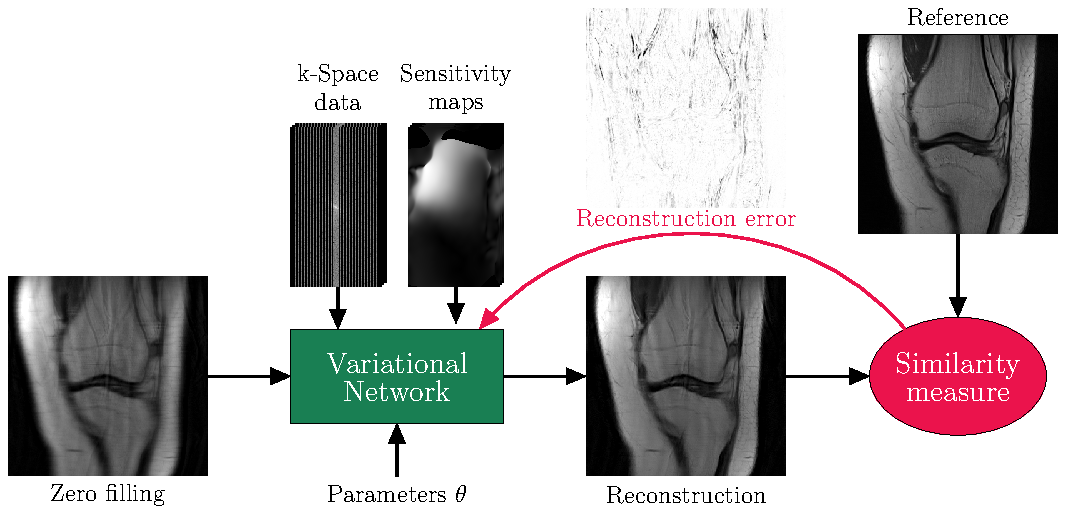
\includegraphics[width=1.0\textwidth]{../Common_Images/varnetworks/figure2-training_overview.pdf}
    \caption{Training overview for a Variational Network. A dataset of undersampled clinical measurements $f_s^\delta$ and fully sampled gold-standard references $u_s$ is used to optimise the network parameters $\Theta$ over unrolled iterations, minimising the loss function outlined in Equation \eqref{eq:hammernik_loss}. Image taken from \cite{hammernik2018learning}.}
    \label{fig:vn_training_overview}
\end{figure}

Crucially, the success of this clinical Variational Network is anchored in how it constraints the learning problem to only the regularisation model. Hammernik et al. structured the unrolled layers strictly as a trainable Field of Experts (FoE) \cite{roth2005fields} model, mathematically analogous to the parametric regulariser introduced in Equation \eqref{eq:foe_model}. Furthermore, by setting the potential functions as convex combinations of radial basis functions, the learned regulariser becomes highly interpretable. 

Instead of deriving opaque feature maps, reading the trained network's explicit linear filters reveals easily recognizable, human-parsable motifs -- such as directional Gabor-like filters and finite-difference operators. These intuitively act as non-linear, orientation-specific variants of Total Generalised Variation (TGV), as detailed in Example \ref{exm:tgv_inv}, promoting piece-wise smooth image regions without blurring sharp tissue boundaries. Figure \ref{fig:clinical_mri_learned_filters} visualises these learned clinical MRI filters.

\begin{figure}[htpb]
    \centering
    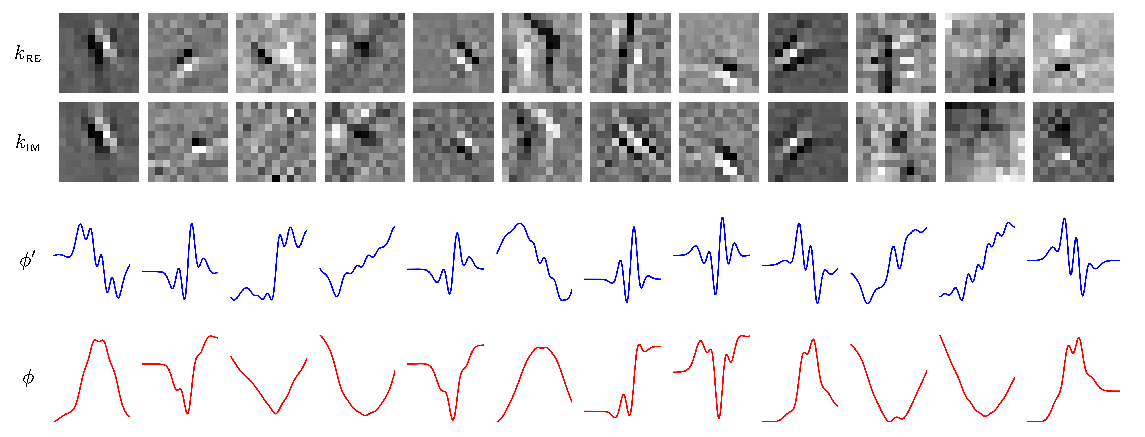
\includegraphics[width=0.8\textwidth]{../Common_Images/varnetworks/figure9-parameters.pdf}
    \caption{Visualisation of the learned complex-valued convolutional filters $D_i$ in the clinical MRI Variational Network. The transparent, explicit formulation allows researchers to inspect these kernels directly, revealing edge-detectors and Gabor-like frequency isolators. Image taken from \cite{hammernik2018learning}.}
    \label{fig:clinical_mri_learned_filters}
\end{figure}

Hammernik et al. demonstrated that this VN architecture, restricted to $T=10$ stages, achieves state-of-the-art reconstructions of clinical knee MRIs in just 193 ms per 2D slice. More fundamentally, because the network enforces the physical forward operator $K$ continuously at each unrolled step (via data fidelity skip connections) rather than learning it from scratch, the VN exhibits great generalisation capacity. 

In clinical trials, the network reliably reconstructed unique clinical pathologies -- such as rare bone cysts and complex meniscal tears—that were entirely absent from the training dataset. By treating deep learning as a highly-parametrised regularisation method solving an inverse problem, the VN effectively avoids some of the aggressive hallucination phenomena commonly crippling pure black-box convolutional neural networks (e.g., U-Nets) \cite{hammernik2018learning}. This robust preservation of unseen pathology is illustrated in Figure \ref{fig:pathology_generalisation}.

\begin{figure}[htpb]
    \centering
    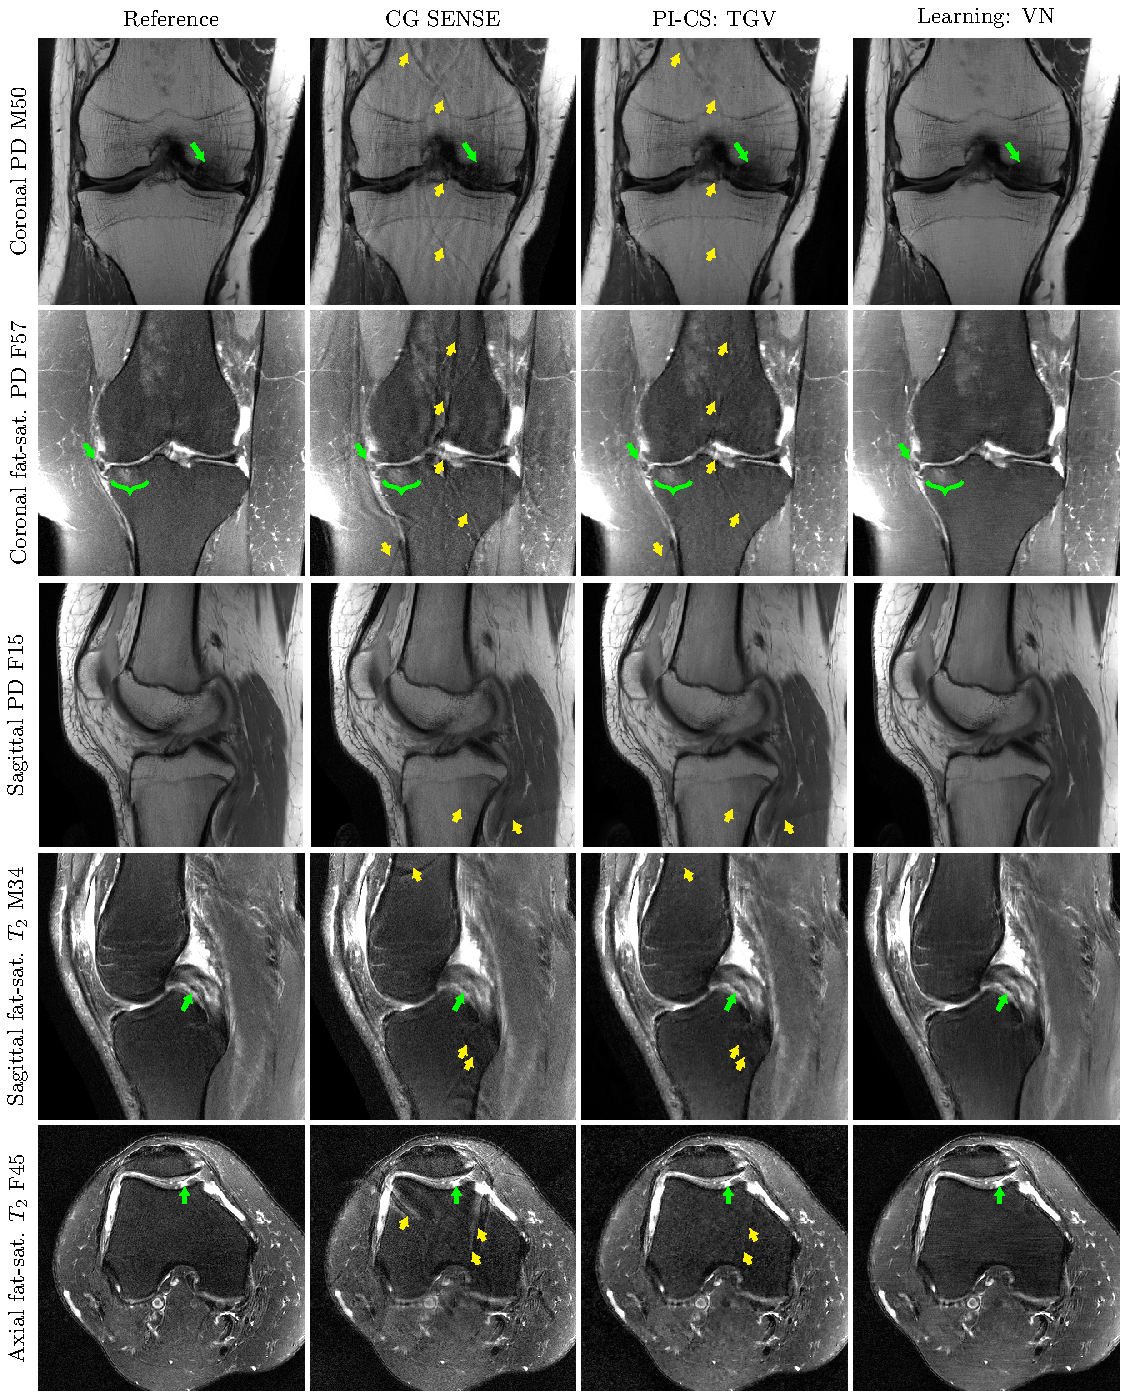
\includegraphics[width=1.0\textwidth]{../Common_Images/varnetworks/figure7-result_kneeprotocol.pdf}
    \caption{Generalisation capabilities of the Variational Network. Despite never having seen a specific meniscal tear during training, the $T=10$ VN successfully reconstructs the exact pathology by relying on rigorous unrolled gradient descent data consistency updates, outperforming baseline U-Nets that tend to hallucinate away unseen geometric anomalies. Image taken from \cite{hammernik2018learning}.}
    \label{fig:pathology_generalisation}
\end{figure}


\section{The Early Stopping Paradox and Optimal Control in VNs}
\label{sec:early_stopping}

In classic variational image processing, researchers have long observed a counter-intuitive phenomenon: strictly converging to the global minimum of a regularised energy functional $E(u)$ often yields worse image quality than stopping the iterative minimisation algorithm early \cite{effland2020variational}. This is commonly observed with hand-crafted regularisers such as the Total Variation model as introduced in Example \ref{exm:rof_inv}. Iteratively descending the gradient initially removes noise, but eventually begins to destroy true structural image textures, leading to artificial ``staircasing'' effects. This is illustrated in Figure \ref{fig:rof_sequence}, where the peak signal-to-noise ratio drops if the gradient steps continue infinitely. 

\begin{figure}[htpb]
    \centering
    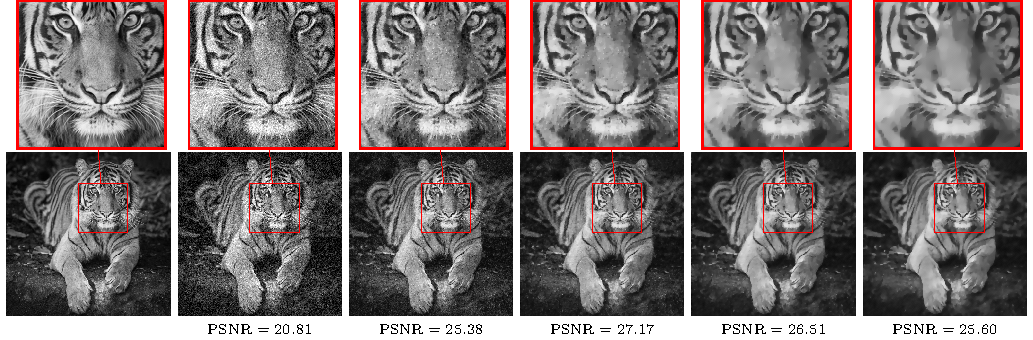
\includegraphics[width=1.0\textwidth]{../Common_Images/varnetworks/fig2.pdf}
    \caption{The Early Stopping Paradox on TV-$L^2$ denoising. From left to right: input image, noisy continuous image, and restored images after 13, 26, 39, and 52 iterations of a gradient descent scheme. The optimal visual and mathematical fidelity peaks at 26 iterations; further gradient steps begin introducing blocky staircasing artifacts, proving that finite halting is structurally necessary. Image taken from \cite{effland2020variational}.}
    \label{fig:rof_sequence}
\end{figure}

This ``early stopping paradox'' persists even in modern Variational Networks. It occurs because even highly expressive, data-driven regularisers cannot perfectly model the true, infinite-dimensional manifold of natural images. Consequently, there is an inherent trade-off between rigorous optimisation and modelling errors. As the number of network layers (iterations) goes to infinity, modelling errors compound, and the reconstruction degrades. Thus, ensuring an ideal ``finite depth'' for our VNs becomes paramount.

\subsection{Stopping Time as a Control Parameter}

Rather than relying on heuristic early stopping rules or treating the architectural number of unrolled layers $T$ as an arbitrary hyperparameter, Effland et al. \cite{effland2020variational} demonstrated that VNs can be formulated seamlessly as a continuous optimal control problem, precisely as we derived for standard Residual Networks in Section \ref{sec:optimal_control}. By doing so, the stopping time $T$ acts directly as an explicit, learnable control parameter alongside $\Theta$.

We define the state equation as the continuous gradient flow of the Variational Network energy functional. If we employ the time-reparameterisation technique $x(t) = u(tT)$, we can map the integration bounds to exactly $t \in (0, 1)$, pushing the stopping time $T$ continuously into the system dynamics. The autonomous state ODE then takes the generalized form
\begin{equation}
    \frac{d}{dt}x(t) = T \mathcal{F}(x(t), \Theta) = T \left( -K^*(Kx(t) - f^\delta) - \sum_{k=1}^{N_D} (D_k)^\top \rho_k'\left(D_k x(t)\right) \right) \, ,
    \label{eq:effland_state}
\end{equation}
with the initial condition $x(0) = u_0$. Here, our optimal control challenge is that we seek to find the optimal scalar stopping time $T$ and the neural network parameters $\Theta$ that minimise the discrepancy between the final evaluated state at $t=1$ and the exact ground truth $u^\dagger$, formalised by the trajectory cost functional $\mathcal{J}(x(1)) = \frac{1}{2}\|x(1) - u^\dagger\|_2^2$.

\begin{figure}[htpb]
    \centering
    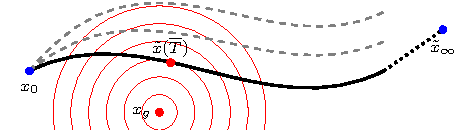
\includegraphics[width=0.7\textwidth]{../Common_Images/varnetworks/fig3.pdf}
    \caption{Schematic of a continuous state trajectory generated by the derived energy functional. The optimal control objective seeks the exact stopping time $\overline{T}$ where the continuous trajectory is closest tangentially to the ground truth $x_g$ (marked by the innermost red concentric isolation line), dynamically avoiding the infinitely smooth, mathematically stationary trap sink $\tilde{x}_\infty$. Image taken from \cite{effland2020variational}.}
    \label{fig:trajectory_topology}
\end{figure}

\subsection{First and Second-Order Optimality Conditions}

To automatically calculate this energy-minimising optimal stopping time via deep learning primitives, we construct the Lagrangian by adjoining the reparameterised state equation \eqref{eq:effland_state} using the time-dependent, backward-in-time adjoint state $p(t)$. By evaluating the variation of the Lagrangian strictly with respect to the scalar horizon multiplier $T$, we recover the rigorous first-order necessary condition
\begin{equation}
    \int_0^1 \left\langle p(t), \frac{d}{dt}x(t) \right\rangle \, dt = 0 \, .
    \label{eq:effland_first_order}
\end{equation}
The continuous adjoint state $p(t)$ solves an associated backward-time ODE coupled with standard backpropagation gradients and initialised via the terminal condition $p(1) = x(1) - u^\dagger$, similar to the optimal control derivation in Section \ref{sec:optimal_control}. Equation \eqref{eq:effland_first_order} elegantly states that at the continuous global minimum of stopping time $T$, the integral product between the network's forward ODE velocity and the adjoint error gradient field must be perfectly structurally orthogonal \cite{effland2020variational}.

\begin{figure}[htpb]
    \centering
    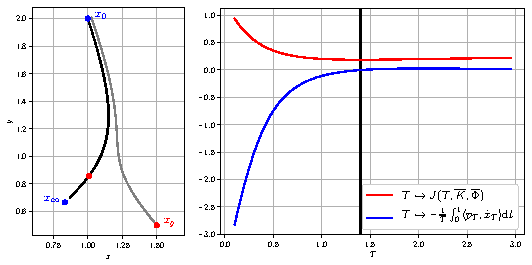
\includegraphics[width=1.0\textwidth]{../Common_Images/varnetworks/fig4.pdf}
    \caption{Visualisation of the continuous first-order optimality objective mapping exactly to the early stopping phenomenon. The first order condition $\int \langle p, \frac{d}{dt}x \rangle$ strictly evaluates to $0$ precisely at the minimum value identically mapped to the system's global $L^2$ trajectory metric. Image taken from \cite{effland2020variational}.}
    \label{fig:optimal_time_plots}
\end{figure}

To guarantee that this optimal time $T$ acts stably as a local minimum (verifying that increasing depth further will natively harm performance), one can evaluate a strict second-order sufficient gradient condition ensuring strict positivity across the local curvature field. By jointly optimising parameters $\Theta$ alongside $T$, the continuous network architecture dynamically derives its optimal depth natively from structural data gradients. 

\subsection{Connection to Discretised Static Networks}
By taking the perfectly continuous state equation \eqref{eq:effland_state} representing our explicit Variational framework, we easily derive standard neural architectures simply by running explicit numerical integration templates. A simple forward Euler time discretisation across a uniform set of nodes yielding step sizes of $\Delta t = T/S$ directly gives the update schema $x_{s+1} = x_s + \frac{T}{S} \mathcal{F}(x_s, \Theta)$. 

These models are functionally equivalent to deep Residual Networks where parameters $\Theta = \{D_k, w_{jk}\}$ are static (shared identically) across layers, commonly termed Static Variational Networks \cite{effland2020variational}. Consequently, by controlling the discretisation size explicitly relative to the theoretical horizon $T$, Variational architecture designers map deep network layers conceptually and computationally identically to robust Runge-Kutta numerical solvers over physical operator equations.

\subsection{Nonlinear Spectral Dynamics}

Why does the network flow formally improve the imaging structures before halting safely, rather than indiscriminately destroying the picture? Effland et al. \cite{effland2020variational} studied this by analysing the gradient of the highly-parameterised field-of-experts model specifically via nonlinear eigenvalue problems of the form
\begin{equation}
    \sum_{k=1}^{N_D} D_k^\top \rho_k'(D_k v) = \lambda v \, .
\end{equation}

Extracting the generalised eigenfunctions $v_j$ corresponding to various eigenvalues $\lambda_j$ unravels exactly what the discretised layers dynamically evaluate. Looking at the explicitly discretised solver update scheme with $T/S$ step-sizes mapping to the regulariser, modifying an evaluated eigenfunction yields $v_j - \frac{T}{S} (\lambda_j v_j) = (1 - \lambda_j \frac{T}{S}) v_j$. 

\begin{figure}[htpb]
    \centering
    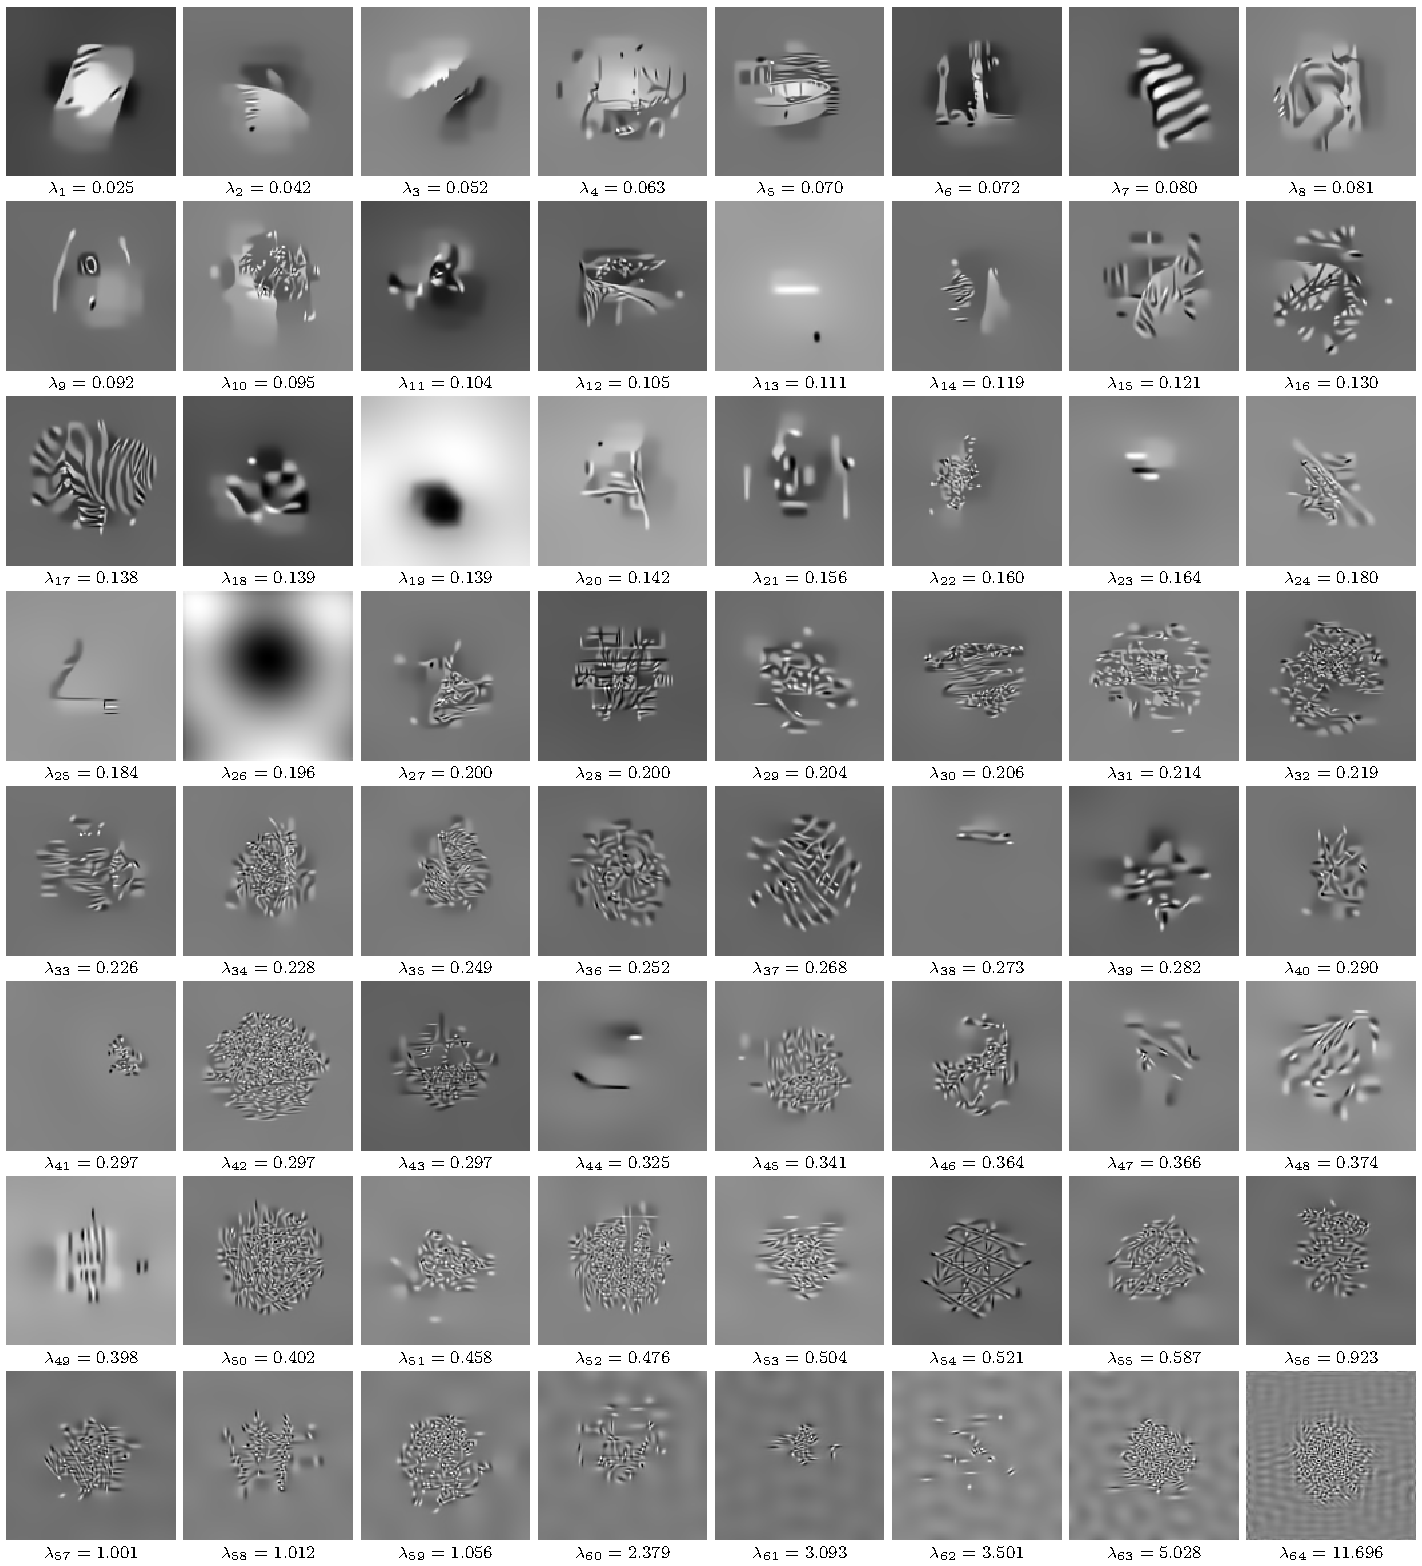
\includegraphics[width=1.0\textwidth]{../Common_Images/varnetworks/fig13.pdf}
    \caption{Computed general eigenpairs modeling the interior dynamics of the learned Variational filter. Lower eigenvalue coefficients $\lambda$ match large-scale cartoon-like structures and tissue boundaries, shielding them organically from strong attenuation. Extreme high eigenvalues identify almost exclusively to granular, noisy spatial structures matching aggressive systemic attenuation. Image taken from \cite{effland2020variational}.}
    \label{fig:eigenpairs_denoising}
\end{figure}

The analysis reveals that eigenfunctions structurally matching high-frequency, noisy scatter patterns inherently produce very large eigenvalues (implying heavy damping where the attenuation factor sharply contracts). Conversely, key structural boundaries and textures yield exceedingly small $\lambda$ values near $0$, yielding an contraction factor structurally matching approximately $1$. Thus, the continuous optimal control framework demonstrates that deep network layers theoretically function identically to sophisticated, nonlinear dynamic spectral filters: rapidly annihilating statistical noise within the first gradient layers, whereby the learned optimal stopping time $T$ acts to halt network flow uniformly before the more slowly decaying macro-structures are being smoothed out.